\chapter{Metodologia}
\label{chap:metodologia}

O propósito dessa seção é especificar como o trabalho foi realizado, apresentando o tipo de pesquisa, o meio de coleta de dados, o cenário e a análise dos dados coletados a fim de atingir os objetivos propostos.

\section{Fluxo de Desenvolvimento}
\label{sec:fluxo-de-desewnvolvimento}

A figura \ref{fig:fluxo} mostra o fluxo utilizado para o desenvolvimento deste trabalho.

\begin{figure}[h!]
	\centering
	\Caption{\label{fig:fluxo} Fluxograma do processo}	
	\UNIFORfig{}{
		\fbox{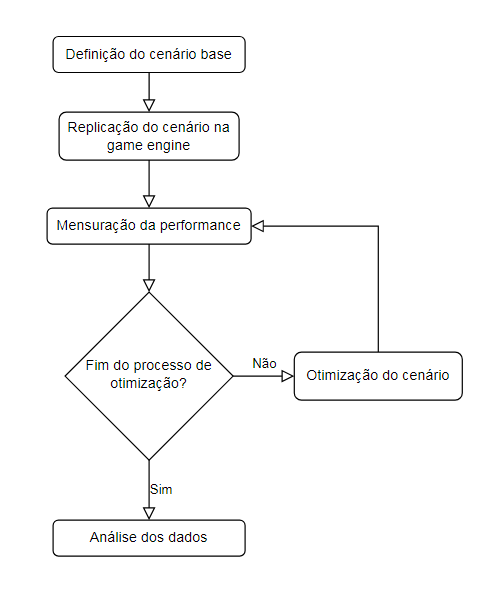
\includegraphics[width=9cm]{figuras/fluxo}}
	}{
		\Fonte{Elaborado pelo autor (2021)}
	}	
\end{figure}

\section{Sobre a pesquisa}
\label{sec:sobre-a-pesquisa}

A pesquisa realizada para a elaboração do presente trabalho é do tipo aplicada, por se tratar de um estudo de análise comparativa e que propõe gerar conhecimento. Esse é um tipo de pesquisa que envolve estudos profundos com a intenção de resolver problemas presentes no em um contexto social semelhante ao dos pesquisadores (GIL, 2017)\nocite{pesquisa}.

Em relação a classificação da pesquisa, pode-se constatar que trata-se de um estudo com características exploratórias por proporcionar maior familiaridade com o problema e descritivas por focar nas características do objeto de estudo (GIL, 2017). Sua finalidade é portanto de criar e ampliar pressuposições, elucidar informações e incertezas sobre o assunto e complementar os entendimentos do expolorador.

Já quanto ao tipo de abordagem, seguindo a definição de Hernandez et. al. (2013)\nocite{hernandez2013}, entende-se que é do tipo quantitativa por ocorrer por meio da coleta de dados para teste de hipóteses baseando-se na medição numérica e na análise estatística para comprovar teorias e estabelecer padrões. Na abordagem quantitativa, os resultados são propagados por meio de quantitativos adquiridos no processo de coleta dos dados.

Conforme Marconi e Lakatos (2019)\nocite{marconi2019}, a investigação bibliográfica é feita pela pesquisa e exposição de bibliografias públicas (livros, revistas, artigos, teses), para mostrar com profundidade os assuntos delimitados pelo pequisador. A pesquisa bibliográfica, dessa forma, ajuda a obter resultados expressivos no estudo desenvolvido. 

\section{Escolha das \textit{game} \textit{engines}}
\label{sec:escolha-das-game-engines}

Em relação a Unity, é a \textit{engine} mais popular entre desenvolvedores de jogos (motor mais popular na plataforma de jogos Steam), especialmente para projetos pequenos e médios. Alguns jogos populares desenvolvidos com ela são: Fall Guys, Among Us, Phasmophobia e Cities (DOUCET; PECORELLA, 2021)\nocite{lars2021}.

Já sobre a Unreal, que cada vez mais reduz as taxas de licenciamento e torna-se mais acessível. Ela é mais propícia para projetos de grande porte (grandes estúdios e jogos AAA). Jogos famosos desenvolvidos com essa engine: ARK, Borderlands, XCOM e PUBG (DOUCET; PECORELLA, 2021).

Por outro lado, a escolha da Godot ocorreu por ser uma \textit{engine} intuitiva, de código aberto, que apresenta diversas funções que facilitam o desenvolvimento de jogos e por apresentar um crescimento de popularidade e de uso entre desenvolvedores (VARGAS, 2020)\nocite{vargas2020}. 

\section{Sobre os dados e características}
\label{sec:sobre-os-dados}

Neste trabalho, os dados necessários para a realização do \textit{benchmarking}, como taxa de quadros e tempo de execução, foram obtidos a partir da execução das ferramentas de \textit{profiling}. Pois são dados que são obtidos em tempo real. Esses dados foram analisados para os \textit{shaders} utilizados no cenário base em cada uma das \textit{game} \textit{engines} levando em consideração múltiplos níveis de otimização.

Em relação as características de hardware, foi utilizado um computador com sistema operacional Windows 7 Ultimate, processador Intel(R) Core(TM) i3-2120 CPU @ 3.30GHz, memória RAM de 8 GB, disco rígido de 500 GB, unidade de estado sólido de 120 GB, placa de vídeo PCI Radeon R7 360 e placa mãe com chipset H61.

A cena padrão de testes foi estabelecida por meio do uso de um conjunto de objetos 3D para caracterizar um teste de estresse pelo uso de várias malhas com bastantes triângulos. A Tabela \ref{qua:cenaTeste} contém as quantidades de elementos contidos na cena.

\begin{table}[h!]
	\Caption{\label{qua:cenaTeste} Contagem de elementos presentes na cena de teste}\UNIFORqua{}{
	\begin{tabular}{|l|c|c|c|} \hline
		            & Vértices  & Triângulos & Qtd.  \\ \hline
		Casa        & 6901      & 4264       & 72    \\ \hline
		Plano       & 4         & 2          & 144   \\ \hline
		Árvores     & 794       & 368        & 288   \\ \hline
		Cercas      & 7156      & 3632       & 360   \\ \hline
		Cogumelos   & 2208      & 1056       & 360   \\ \hline
		Rochas      & ---       & ---        & ---   \\ \hline
		~Tipo 1     & 576       & 338        & 432   \\ \hline
		~Tipo 2     & 554       & 338        & 144   \\ \hline
		~Tipo 3     & 690       & 426        & 288   \\ \hline
		~Tipo 4     & 512       & 280        & 216   \\ \hline  
		~Tipo 5     & 120       & 62         & 72    \\ \hline
		Água        & 8         & 12         & 4     \\ \hline
		Soma        & 19523     & 10778      & 2380 \\ \hline
		Total       & 46464740  & 25651640   & ---   \\ \hline
	\end{tabular} 
	}{
		\Fonte{Elaborado pelo Autor (2021)}
	}
\end{table} 
 